\chapter{Semantic Description of Road Systems}
\label{ch:descriptionOfRoadSystems}
The following chapter provides a thorough description of the models and semantic description generation process for an urban aria from ESRI CityEngine (CE) using data provided by OpenStreetMap (OSM). Moreover, we provide a detailed explanation of the resulting JSON format which holds information about essential scene data. Lastly, we explain how the resulting file is parsed and used by Unity3D. Additionally, we defend design decisions, as well as describe failed attempts in the process.

A general overview of the whole process can be seen in Figure \ref{fig:overview}. Firstly, OSM maps data are sanitised and imported in CityEngine. Afterwards, 3D models are generated together with a semantic road description. In the end, they are imported and utilised in Unity3D. The navigation module which can be seen in \emph{Unity Game Engine} will be discussed in Chapter \ref{ch:gps}.

\begin{figure}[htb]
	\centering
	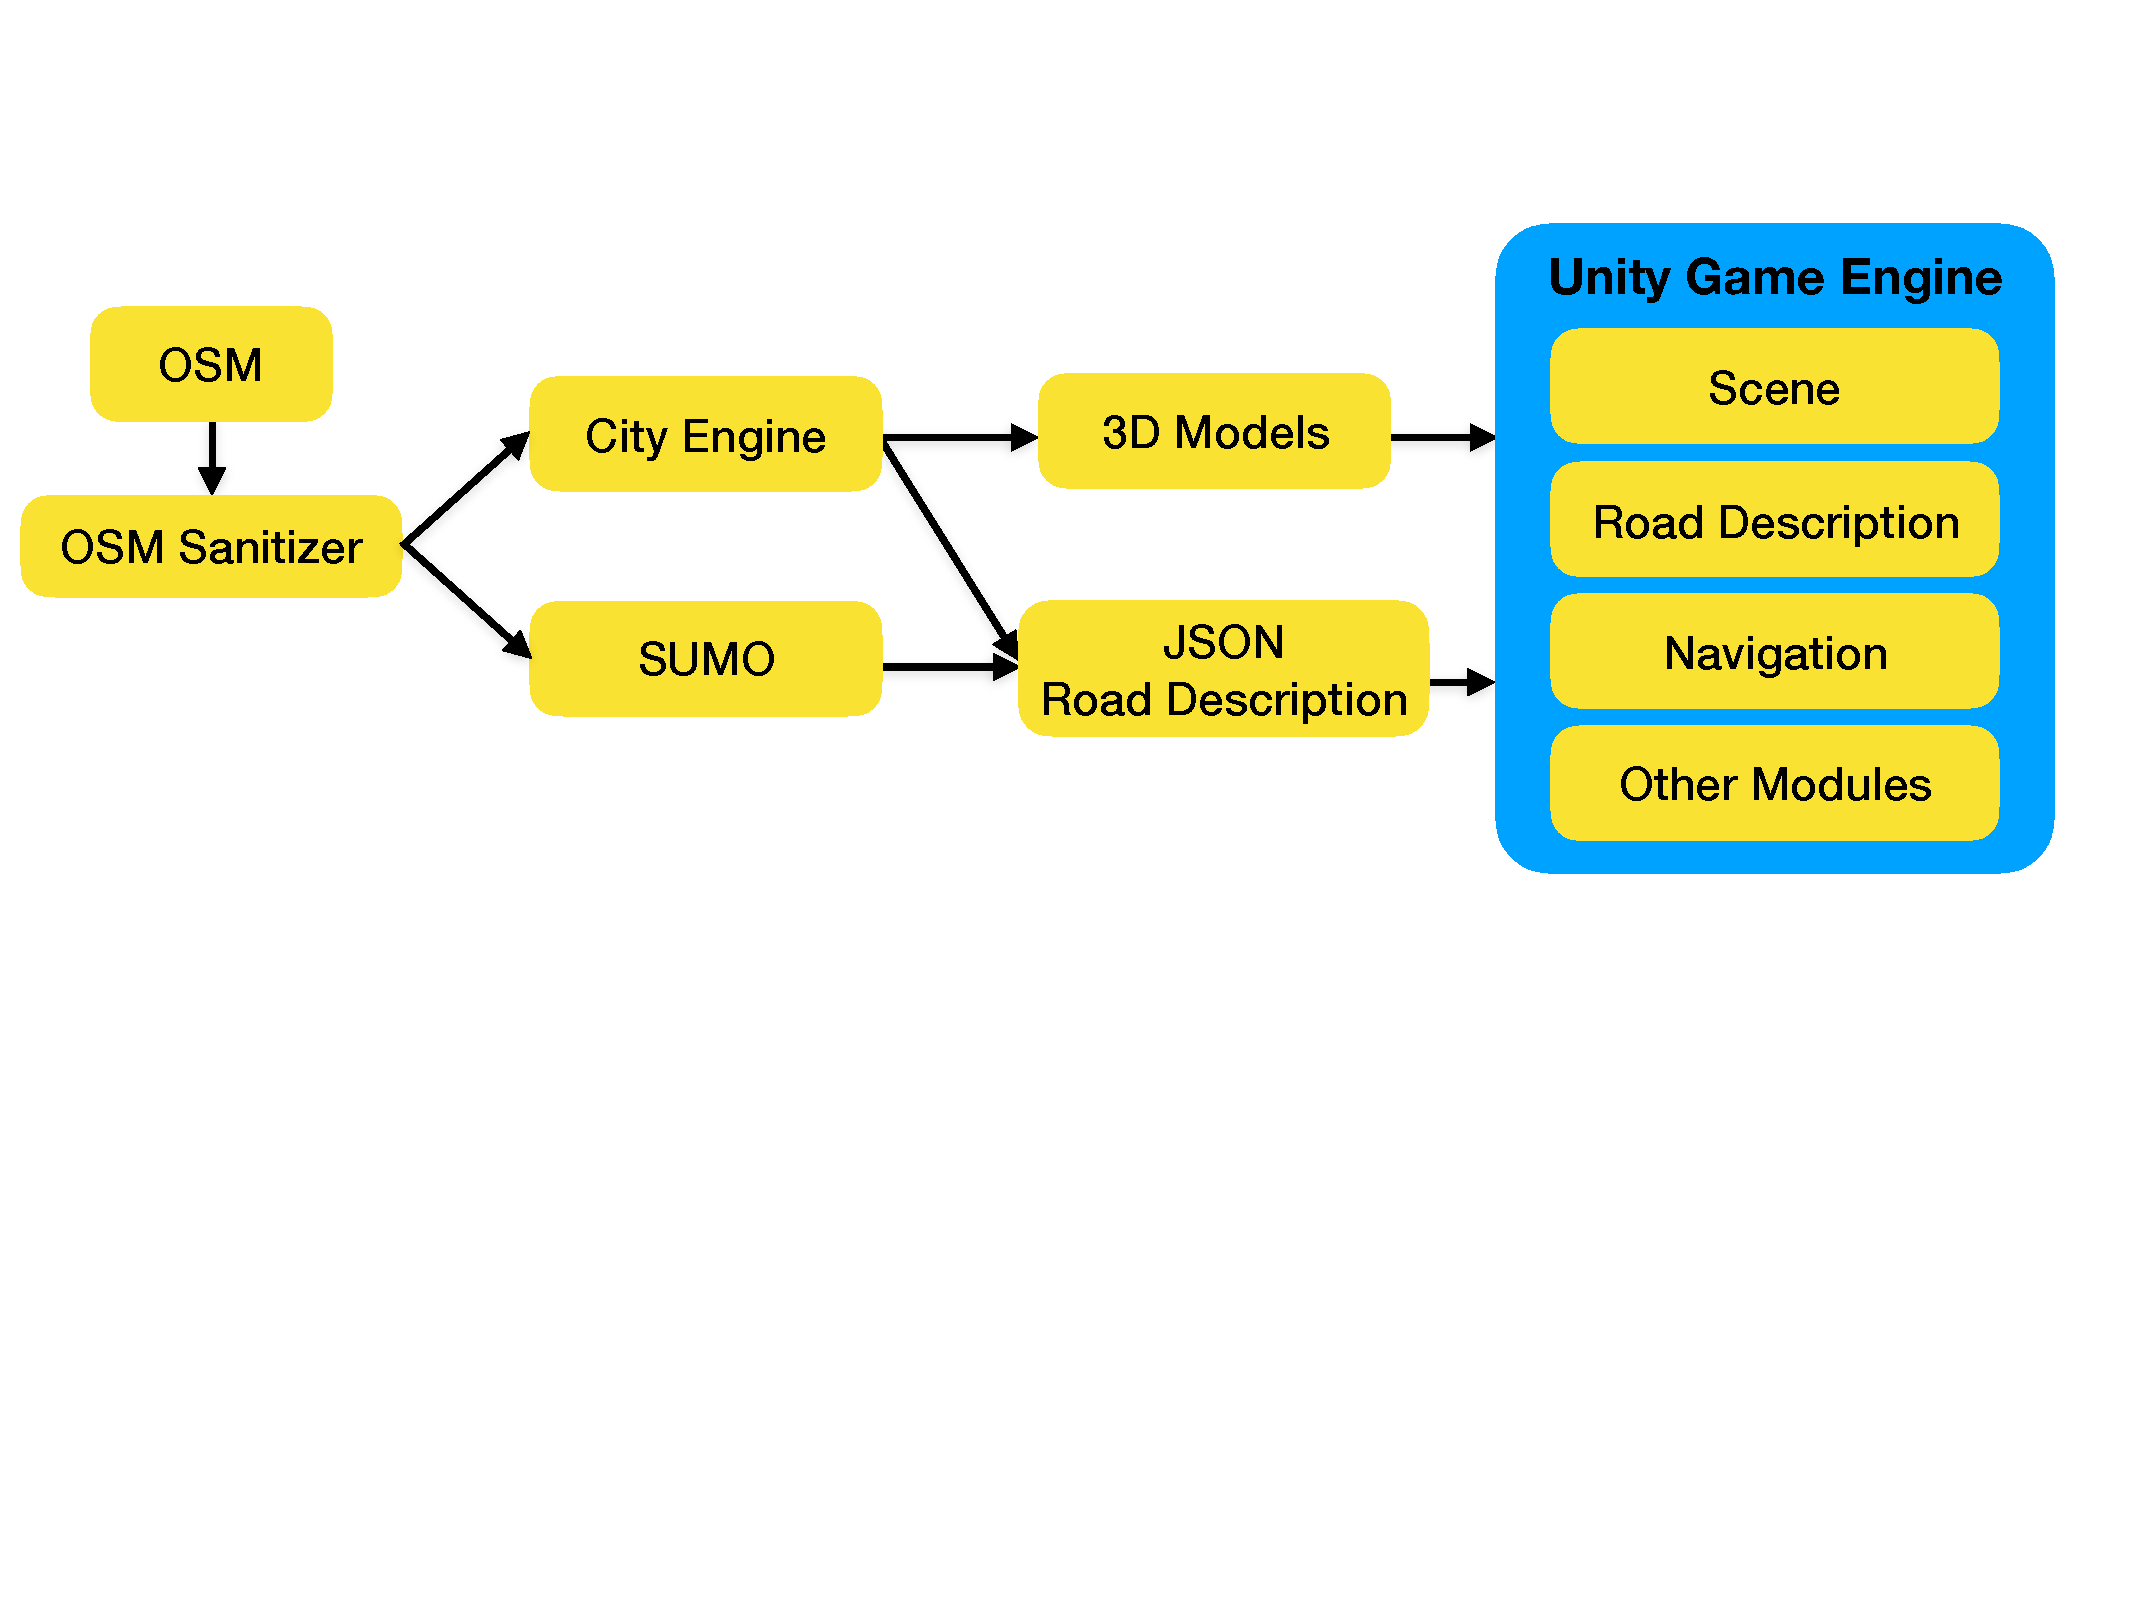
\includegraphics[width=0.95\linewidth]{figures/overview}
	\caption{Overview of the scene creation workflow.}
	\label{fig:overview}
\end{figure}

\section{OSM Export}
As already introduced, the whole map data used in the MMK Driving Simulator is exported from OSM. In Figure \ref{fig:overview} we can see that exported \emph{OSM} file is fed to a \emph{OSM Sanitizer}. There are multiple reasons why this is necessary. Firstly, the objects contained in the export include some unnecessary information which are not present in the simulation, \emph{e.g.} underground network, footpaths. Moreover, this additional objects in the map represent a obstacle for both SUMO and CE when they are building a scene. For example, in Figure \ref{fig:nosimply} and \ref{fig:simply} one could see the difference in the shape creation between respectively a unsanitised and sanitised version of the same \emph{OSM} export data.  

\begin{figure}[htb]
	\centering
	\subfigure[Unsanitised] {
	  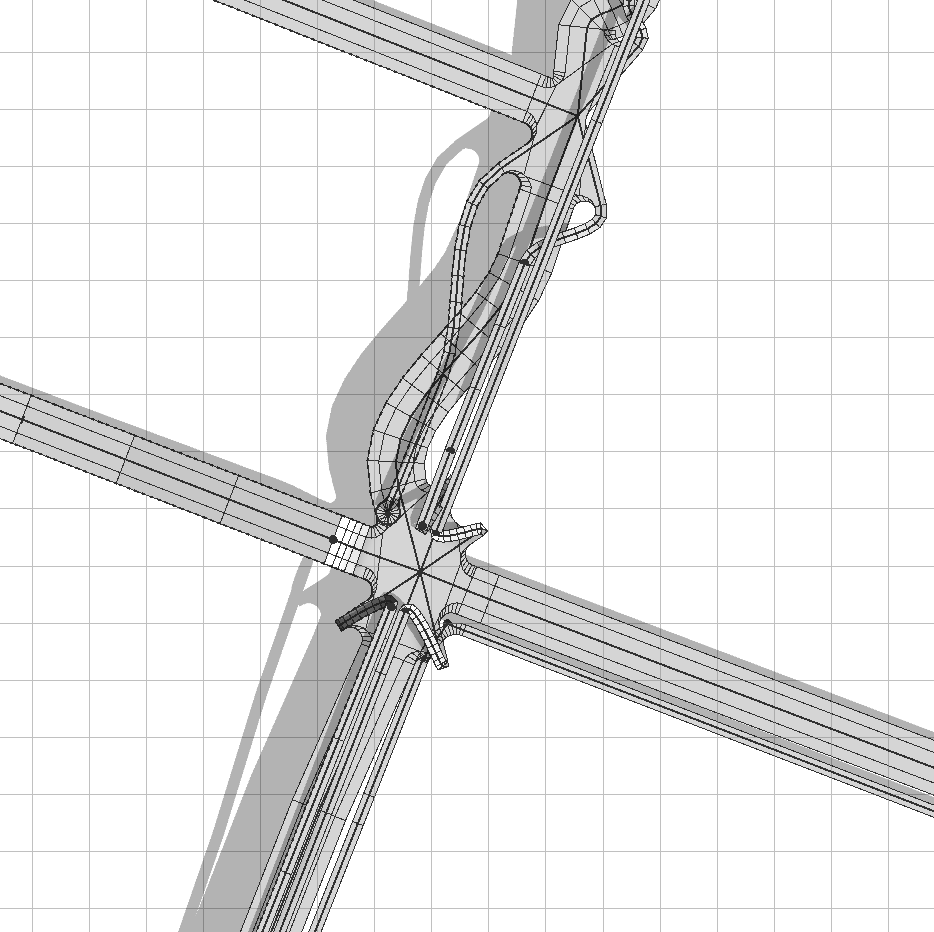
\includegraphics[width=0.4\textwidth]{figures/no-simply}
	  \label{fig:nosimply}
	}\hspace{0.05\textwidth}% \hfill or \hspace{5mm} or \hspace{0.3\textwidth}
	\subfigure[Sanitised] {
	  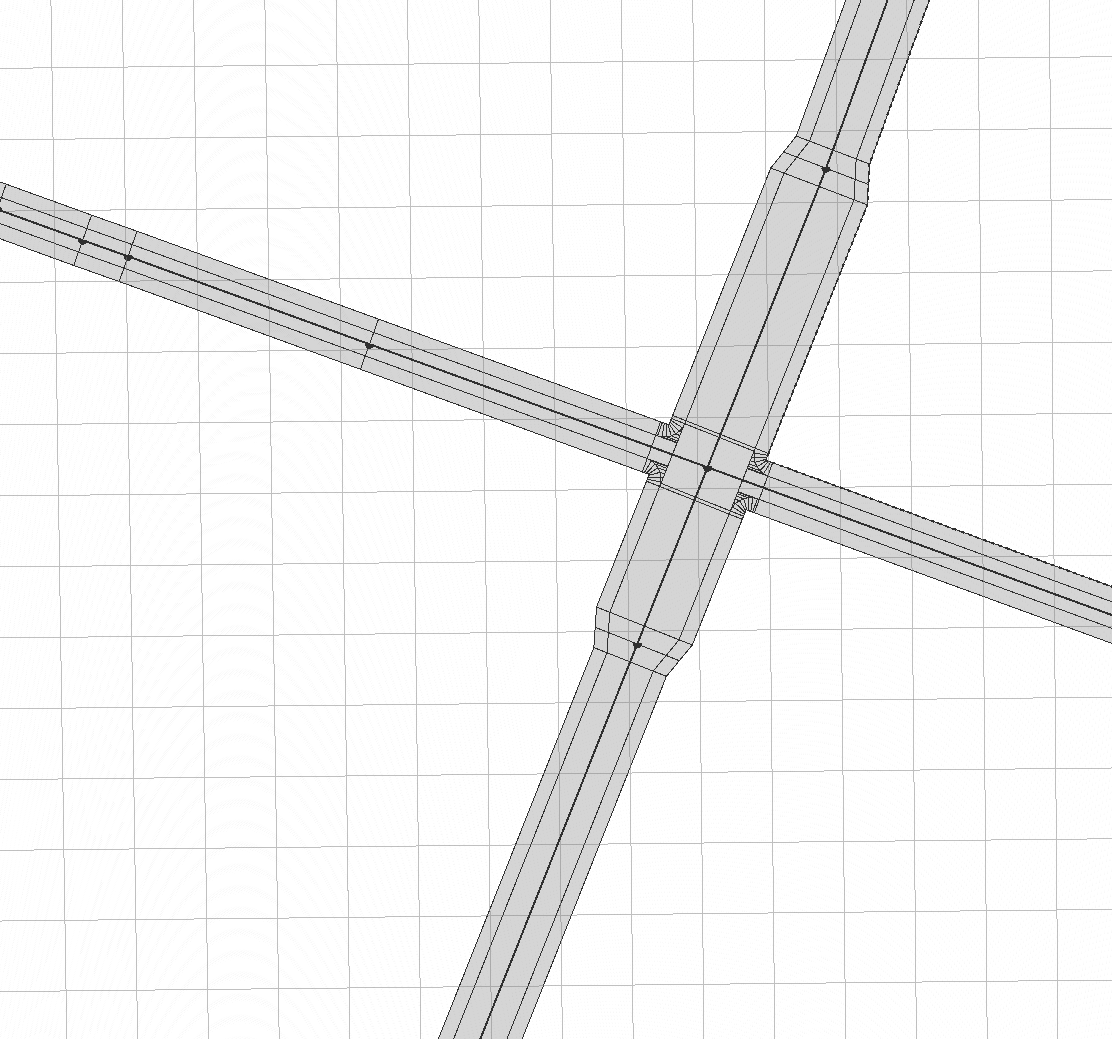
\includegraphics[width=0.4\textwidth]{figures/simply}
	  \label{fig:simply}
	}
	\caption{Comparison of the same CityEngine generated shapes from unsanitised and sanitised \emph{OSM} export file.}
\end{figure}

Since the information in the OSM export is only 2D, CE attempts to to find the perfect location for every shape, although most of them overlap. Therefore, it chooses \texttt{y} values which would generate reasonable shapes. Clearly, the scene generated in this way could not be used in Unity, so we have to delete some of the data. This was achieved by a Python3 script which can be found in \texttt{cityengine-mmk/scripts/osmsanitizer.py}. The script accepts only one input parameter, which is the OSM export file and produces a sanitised version of the same export with the appendix \texttt{-sanitized} in its name.

The sanitisation process follows a straightforward whitelisting fashion. Firstly, we have to delete all roads which are not drivable by a vehicle. Additionally, we want to preserve information about buildings and parkings which should be also present in the export. As we know from Chapter \ref{ch:background}, there are two main objects in OSM which hold information about the infrastructure of the road network: \texttt{way} and \texttt{relation}. According to the OSM documentation\footnote{\url{http://wiki.openstreetmap.org/wiki/Key:highway}}, all streets (\texttt{way} objects) must have a \texttt{highway} tag which marks its type. The valid highway tags are \texttt{motorway}, \texttt{motorway\_link}, \texttt{trunk}, \texttt{trunk\_link}, \texttt{primary}, \texttt{primary\_link}, \texttt{secondary}, \texttt{secondary\_link}, \texttt{tertiary}, \texttt{tertiary\_link}, \texttt{unclassified}, \texttt{residential}, \texttt{living\_street}, \texttt{unsurfaced}. If a \texttt{way} object does not contain a \texttt{highway} tag or the type of the road is not one of the aforementioned fourteen values, then it is deleted. Similarly, we check whether a \texttt{way} object contains a \texttt{building} tag which is set to \texttt{yes} and a \texttt{amenity} tag set to \texttt{parking}. This approach leaves in the OSM export buildings and parkings which coordinates and properties can be later imported in CE.

The sanitiser tries to solve another problem with OSM data, too. Sometimes information about streets, \emph{e.g.} maximum allowed speed or number of lanes, could be missing. When this is the case CE and SUMO try to extrapolate this information and suggest some valid values in order to create the resulting 3D models. Unfortunately, it could happen that both softwares provide different values for the same segment. Because we want to integrate the information streams coming from both, CE and SUMO to create a semantic description of the road network, this data extrapolation has to accomplished one step ahead in the sanitisation process. Therefore, we provide default valid values for missing information and add it to the OSM objects in the final sanitised file.

Finally, we have an OSM data which is valid and contains only the necessary information to build 3D shapes from it. Note that we do not delete any \texttt{node} objects because unused nodes are by default discarded in both, CE and SUMO.

\section{Semantic Description}

\begin{figure}[htb]
	\centering
	\subfigure[] {
	  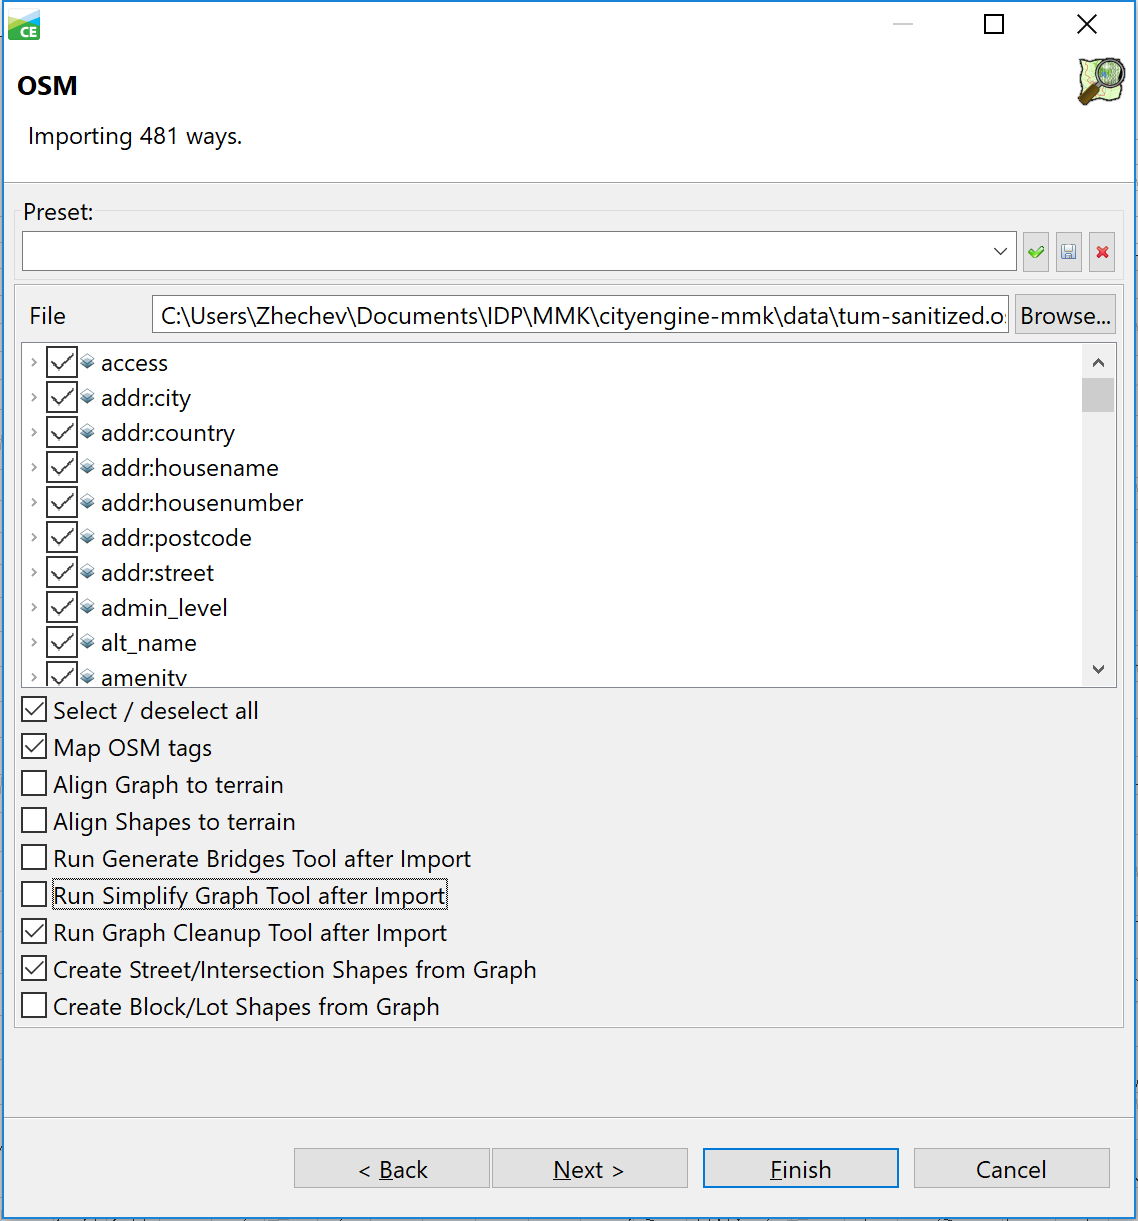
\includegraphics[width=0.28\textwidth]{figures/import}
	  \label{fig:import}
	}%\hspace{0.05\textwidth}% \hfill or \hspace{5mm} or \hspace{0.3\textwidth}
	\subfigure[] {
	  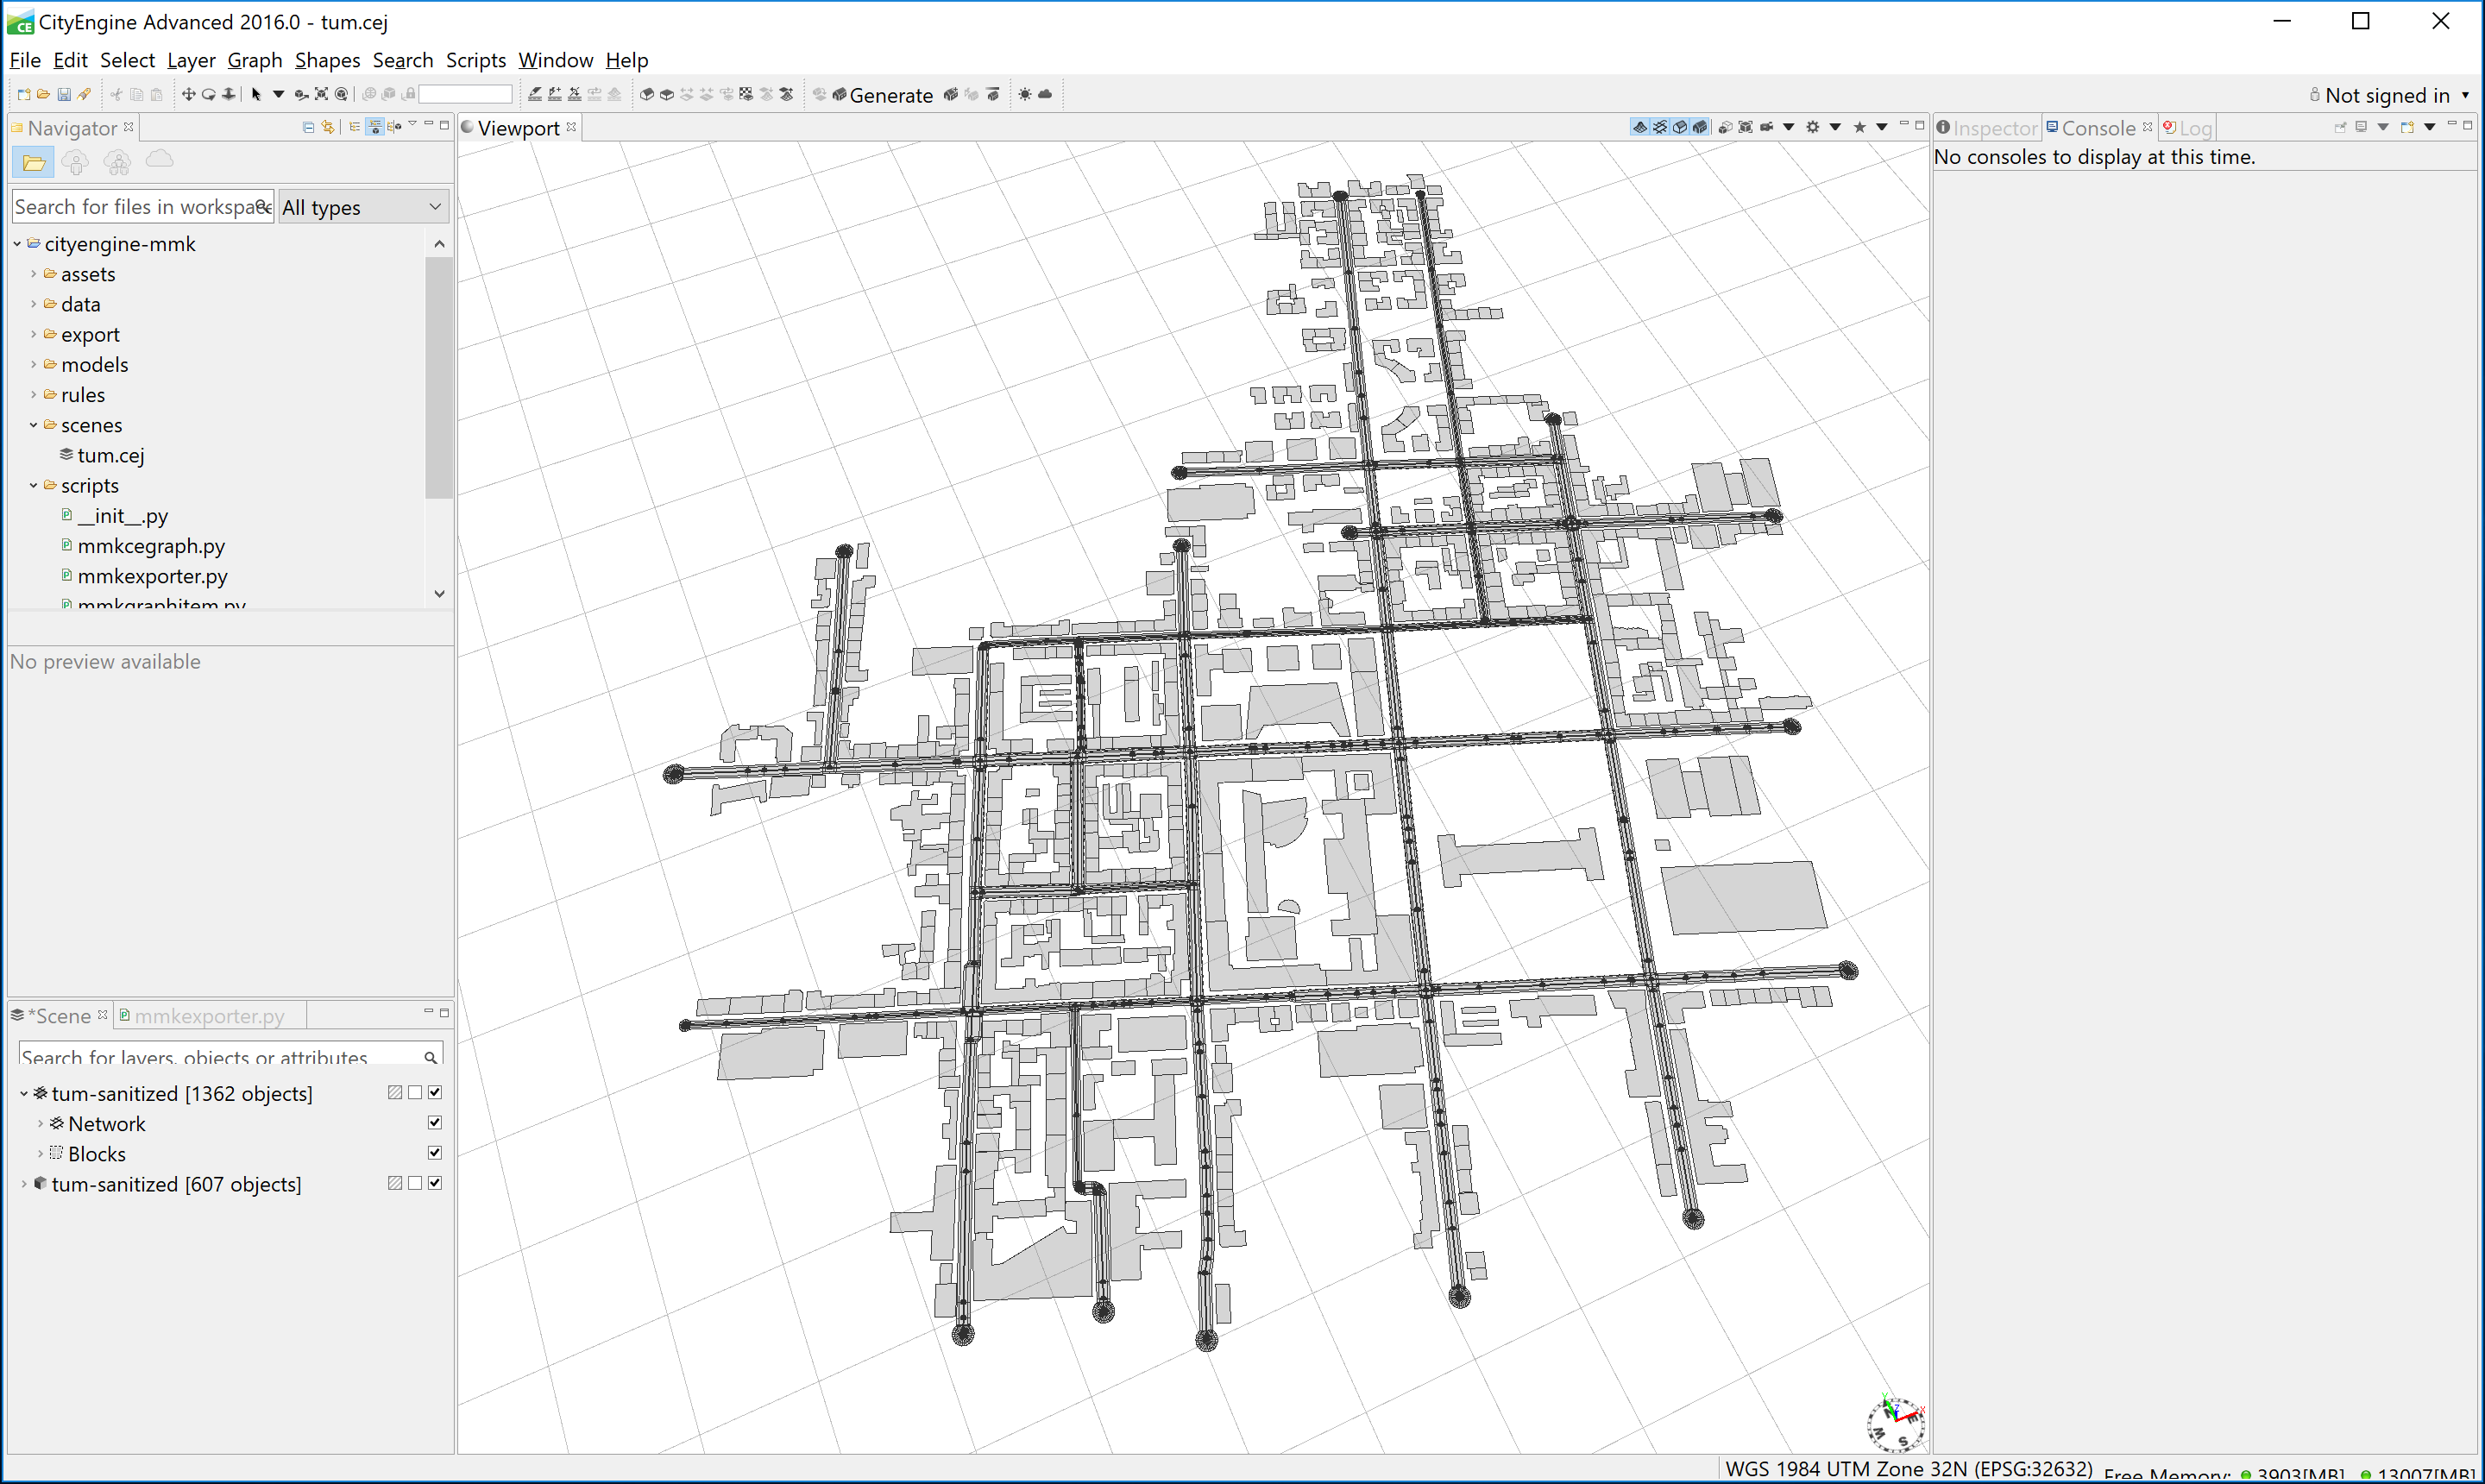
\includegraphics[width=0.68\textwidth]{figures/ce-1}
	  \label{fig:ce-1}
	}
	\caption{}
\end{figure}

\chapter{Car Routing Algorithm}
\label{ch:gps}